\subsection{Ontwerp}

Voor het ontwerp wordt gebruik gemaakt van het 4+1 view-model architectuur zoals beschreven door \cite{kruchten19954+}. Het 4+1 view-model organiseert een beschrijving van een software-architectuur met behulp van vijf gelijktijdige views, die elk een specifieke reeks problemen adresseren.

\begin{wrapfigure}{r}{0.6\textwidth}
  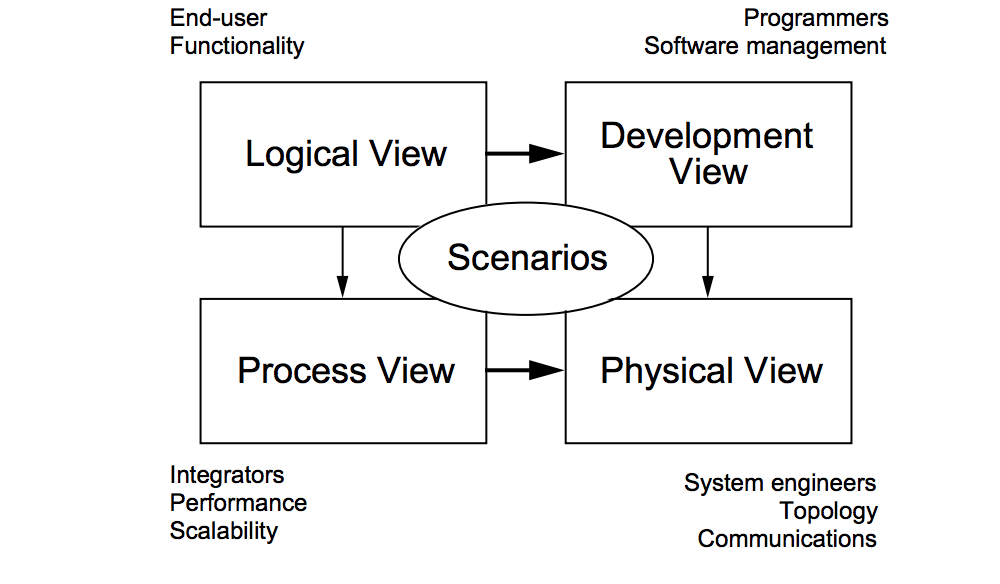
\includegraphics[width=0.6\textwidth, keepaspectratio]{figures/4+1}
  \caption[4+1 view-model]{Het 4+1 view-model volgens \cite{kruchten19954+}.}
  \label{blockchain_architecture}
\end{wrapfigure}

\paragraph{Development view} beschrijft het systeem uit het perspectief van een ontwikkelaar en beschrijft aspecten die te maken hebben met de software matige indeling.

\paragraph{Logical view} beschrijft hoe de eindgebruiker in staat zal zijn om de software te gebruiken. Hierbij worden vaak klassediagrammen en state diagrammen toegepast.

\paragraph{Process view} beschrijft de dynamische aspecten van het systeem op gebied van schaalbaarheid, integratie en performance.

\paragraph{Physical view} beschrijft hoe de softwarearchitectuur gaat werken op de benodigde hardware en focust zich met name op het gedistribueerde aspect ervan.